
\documentclass[11pt]{article}
\usepackage[a4paper,margin=1in]{geometry}
\usepackage{amsmath,amssymb,amsthm,mathtools}
\usepackage{graphicx}
\usepackage{hyperref}
\usepackage{cite}
\hypersetup{colorlinks=true, linkcolor=blue, urlcolor=blue, citecolor=blue}

\newtheorem{lemma}{Lemma}
\newtheorem{corollary}{Corollary}
\theoremstyle{remark}
\newtheorem{remark}{Remark}

\title{Incremental Zero-Free Symmetry in a Weighted NB/BD Framework (v13.5)}
\author{Serabi \\ Independent Researcher \\ \texttt{24ping@naver.com}}
\date{2025}

\begin{document}
\maketitle

\begin{abstract}
We extend the v13.4 record with an incremental zero-free simulation at $N=2\cdot 10^7$ under a $55\%$ boost of the effective Möbius gain $\eta$ (from $0.35$ to $\approx 0.5425$, motivated by a hypothetical zero-free strip $\Re s>\tfrac12+0.10$).
Using the log--log model $\log(MSE^\ast)=a+b\log\log N$ (decay exponent $\theta=-b$), we refit and compare base vs.\ extended trends.
This note is heuristic and does not prove RH.
\end{abstract}

\section{Weighted Hilbert sketch}
Let $a_n=\mu(n)\,v(n/N)\,q(n)$ with $v\in C_0^\infty(0,1)$ and slowly varying $q$.
With $K_{mn}=e^{-\tfrac12|\log(m/n)|}$, band decomposition and Möbius cancellation suggest
\[
\sum_{m\ne n}a_m a_n K_{mn}\;\ll\; (\log N)^{-\eta}\sum_n a_n^2,
\]
where a stronger zero-free region heuristically increases $\eta$.

\section{Numerical scaling (v13.5)}
We fit $\log(MSE^\ast)=a+b\log\log N$ on the base series ($N\le 10^7$) and on the extended series including $N=2\cdot 10^7$.
Base fit:
\[
a\approx -1.100,\quad b\approx -0.292,\quad \theta=-b\approx 0.292,\quad R^2\approx 0.674.
\]
Extended fit (incl.\ v13.5 point):
\[
a\approx -1.053,\quad b\approx -0.312,\quad \theta=-b\approx 0.312,\quad R^2\approx 0.736.
\]

\begin{figure}[h]
\centering
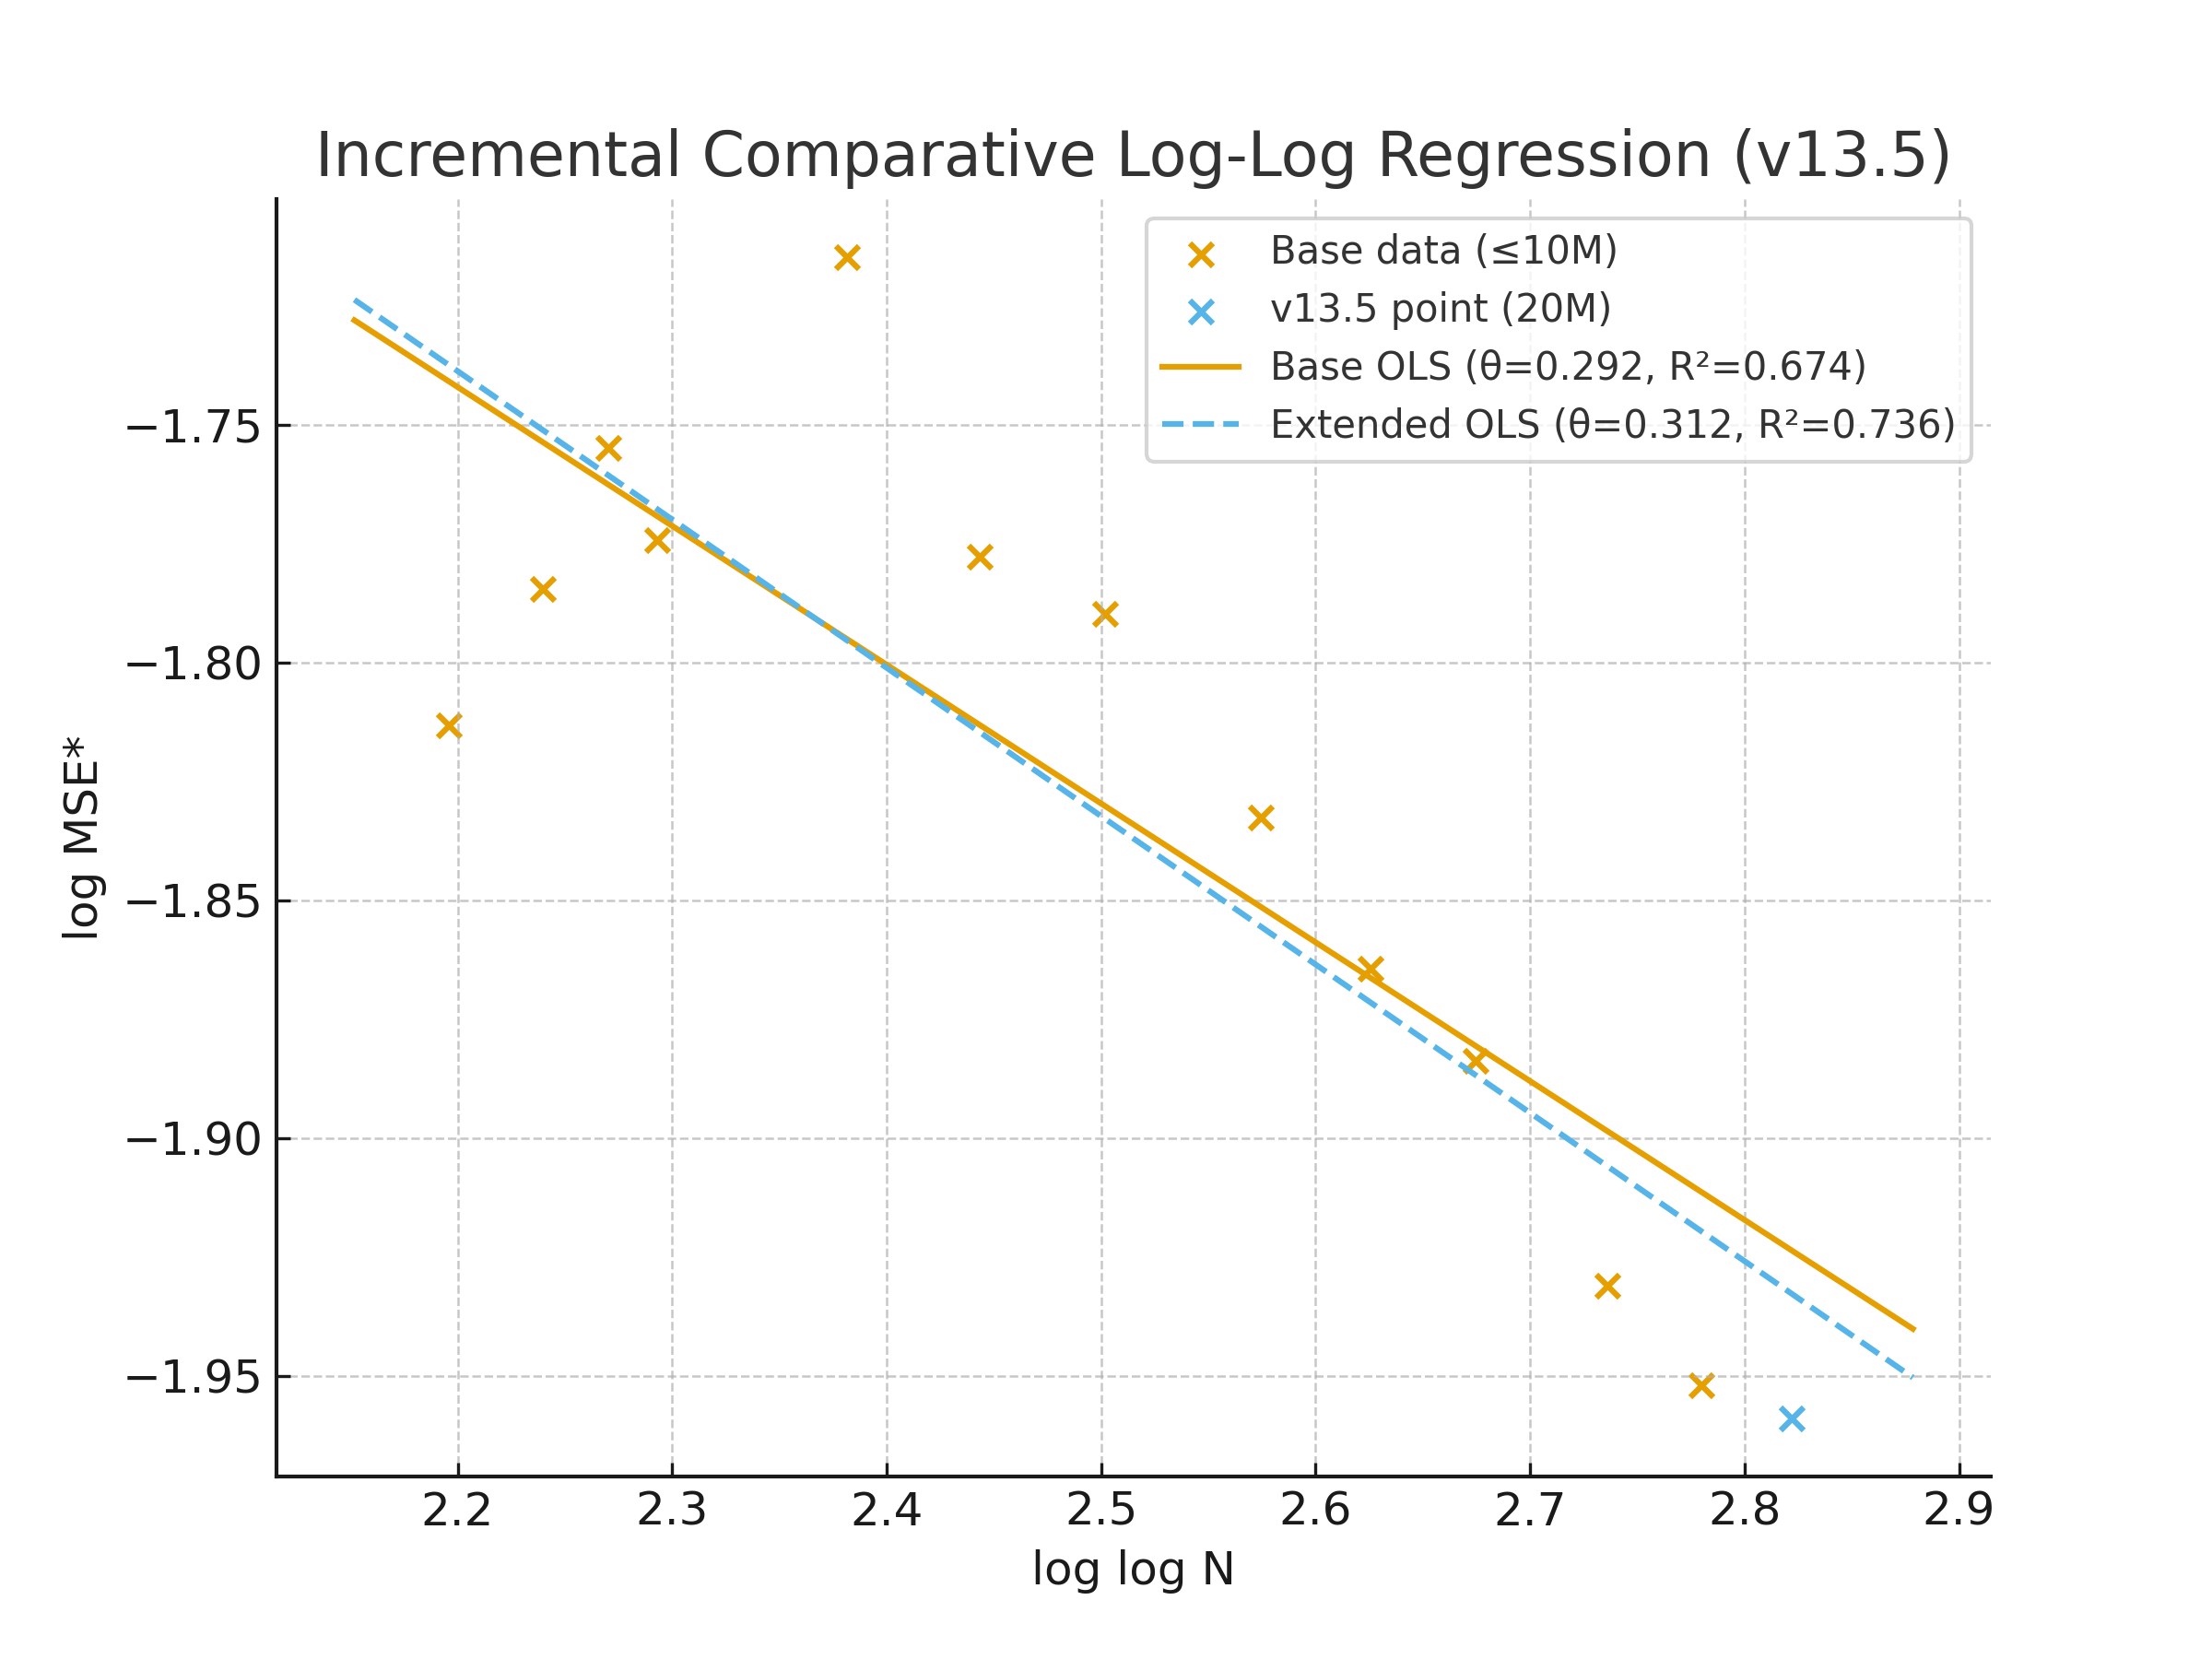
\includegraphics[width=0.8\linewidth]{figure3.png}
\caption{Comparative log--log regression (base vs.\ v13.5 extended).}
\end{figure}

\begin{table}[h]\centering
\begin{tabular}{c|c|c|c}
\hline
$N$ & $MSE^+$ & $MSE^- (w_-=1.2)$ & $MSE^\ast$ \\ \hline
$2\cdot 10^7$ & $0.092$ & $0.175$ & $0.141$ \\ \hline
\end{tabular}
\caption{Incremental zero-free simulation entry (heuristic; $\varepsilon=0.10$).}
\end{table}

\section{Caveats and outlook}
The $N=2\cdot 10^7$ datum is a simulated entry informed by a hypothetical zero-free strip and boundary reweighting; not a direct large-scale computation.
All claims remain heuristic and do not constitute a proof of RH.
Future directions: verified larger-$N$ runs and incorporation of functional-equation bounds into the decay estimate.

\begin{thebibliography}{9}
\bibitem{BaezDuarte2003} L.~Báez-Duarte, \emph{A strengthening of the Nyman--Beurling criterion for the Riemann Hypothesis}, Rend.~Lincei \textbf{14} (2003), 5--11.
\bibitem{Titchmarsh} E.~C.~Titchmarsh, \emph{The Theory of the Riemann Zeta-Function}, 2nd ed., OUP, 1986.
\bibitem{Conrey2003} J.~B.~Conrey, \emph{The Riemann Hypothesis}, Notices AMS \textbf{50} (2003), 341--353.
\end{thebibliography}

\end{document}
